\section{Source Code Repository Mining}\label{lit-repomining}

Source code repository mining refers to the collection and analysis of data from within software source code repositories such as git or CVS, or other historic collections. These repositories are used as a central store of source code and other related artefacts shared between development teams. Changes to these artefacts are made by developers and then ``committed'' to the repository. Information available within the repository commonly includes incremental versions of (or changes to) source code files or other artefacts, such as documentation, along with meta data surrounding changes committed to the repository such as the developer, files changed and comments. This data is seen as a rich potential source of information about software offering the ability to gain comprehension into areas such as the evolution of a software package, bug fixing, semantic relationships between artefacts and developer activity either at a given point in time or mapped over the life of a project \citep{kagdi_survey_2007,allamanis_mining_2013,williams_automatic_2005}.

Although mining is performed most often against source code repositories themselves, other historic sources of information relating to software development are included within the field. These sources, identified in table \ref{tab-lit-repoexample}, may be mined on their own or in conjunction with each other, for example matching source code changes with bug reports \citep{williams_automatic_2005,hassan_road_2008}.

Extraction of data from source code repositories can be complex, as although an increase in open-source projects makes an ever-growing volume of such repositories available to researchers, the repository management software itself is not designed with this type of data collection in mind. Successful extraction and use of data does however continue to grow as does interest in the possibilities inherent in such large collections. In many ways this is demonstrated by the way in which raw data extraction from complex repository formats has now become commonplace and the primary challenge remains how to analyse and use this data to form useful information \citep{hassan_road_2008}.

\begin{table}[H]
\centering
\begin{tabular}{| l | p{8.5cm} |}
\hline
\textbf{Source} & \textbf{Details} \\ \hline

Source Code Repositories & All development history of a project including all changes to files and meta data. May also include large repositories holding information about a number of projects e.g. Sourceforge.net \\ \hline
Bug Repositories & Track the history of bugs including reporting, potentially narrative of investigation, and closure/resolution \\ \hline
Archived Communications & Track interpersonal communication about a project such as mailing lists, chat logs; general archived communications \\ \hline
Deployment Logs & Records of specific deployments for example error or transaction logs \\ \hline


\end{tabular}
\caption{Examples of software repository types \citep{hassan_road_2008,kagdi_survey_2007}}
\label{tab-lit-repoexample}
\end{table}

\subsection{Types of Repository Mining}

Repository mining has often been used to try and comprehend or analyse software evolution over time \citep{kagdi_survey_2007}, as well as in a more applied fashion to improve bug/error detection \citep{williams_automatic_2005} or, of specific interest to this project, to rebuild or refine traceability links between code and documentation  \citep{ali_trustrace:_2013,antoniol_recovering_2002,marcus_recovering_2003,kagdi_mining_2007} or between code artefacts \citep{kagdi_survey_2007}. Before covering traceability recovery in terms of requirements (section \ref{lit-scm-traceability}) and dependencies (section \ref{lit-scm-cocomm}), other main types of repository mining will be identified.

\subsubsection{Understanding and/or Visualising Software Evolution}

Comprehension of large software systems can be a major challenge for organisations and new developers. Many solutions exist to aid in the comprehension of the ``static system'' as it currently is such as reverse engineering (section \ref{lit-reverseengineering}) and technical documentation when available. One use of source code mining is therefore to provide more detailed and historic information about system components including dependencies, enabling their life to be traced and details such the original change commit messages and notes to be recovered \citep{hassan_road_2008}. In a wider context, information from multiple projects can be used to gain insight into the general form of software evolution, how large open-source projects grow and change, and levels of change over time \citep{allamanis_mining_2013,kagdi_survey_2007}.

\subsubsection{Developer or Team Analysis}

Repositories contain meta data concerning who committed changes to what artefacts and when. Not only can this data be used for simple analysis such as the number of active developers or the change in activity patterns over time but, especially in combination with other types of repository such as mailing lists or bug reports, enable the profiling of activity on one or more projects \citep{hassan_road_2008,williams_automatic_2005}.

\subsubsection{Bug Prediction}

The ability to predict and so prevent or mitigate bugs is in many ways one of the ``holy grails'' of software engineering. If such knowledge was available project resources could be more finely targeted and testing focused \citep{hassan_road_2008}. In terms of such analysis \citet{graves2000predicting} found a direct relationship between the number of changes or previous bugs in software with the number of bugs occurring in the future, with more recent changes or bugs being more significant than historic. Use of such metrics as a more effective predictor of bugs compared with traditional complexity measures has also been demonstrated using the codebase from the Eclipse project \citep{moser2008comparative}.

\subsubsection{Enabling and Encouraging Reuse}

Large projects naturally contain large amounts of code. In many cases this is poorly documented or there is a lack of awareness as to the precise content or purpose. This confusing picture does little to encourage reuse with poor visibility of existing APIs or frameworks. Mining of repository data could allow for location of such ``lost'' artefacts for example by identifying previous components in which they have been used and providing the developers with this code and any contemporaneous comments or documentation \citep{hassan_road_2008}.

\subsection{Source Code Mining for Traceability Recovery}\label{lit-scm-traceability}

Recovery of requirements traceability has become an increasing focus of research efforts often focused on rebuilding links between higher and lower level documents within a software system e.g. from documentation to source code. These approaches typically use Information Retrieval (IR) techniques, such as textual comparison, which attempts to find similarities between artefacts at different levels. Performance has been mixed and often generally quite low in terms of balancing both recall (recovered over expected links) and precision (correctly identified links) \citep{ali_trustrace:_2013,antoniol_recovering_2002}. A typical process for text-based IR processing of source and documentation is shown in figure \ref{fig-lit-scm-tracerecovery}.

\begin{figure}[hbtp]
\centering
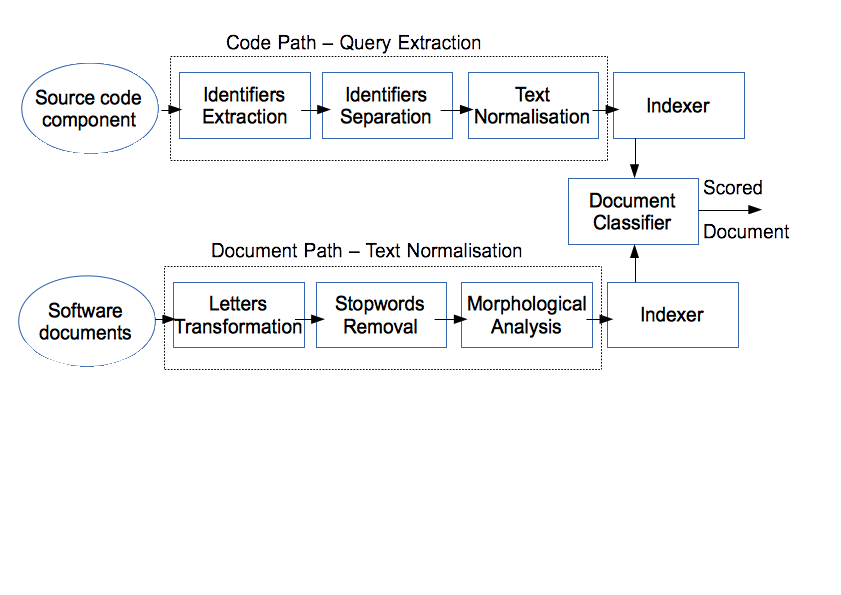
\includegraphics[scale=0.5]{sections/literature/repomining/TLR-Diagram-Antoniol}
\caption{Possible traceability link recovery method \citep{antoniol_recovering_2002}}
\label{fig-lit-scm-tracerecovery}
\end{figure}

One possibility for increasing the performance of traceability recovery is by incorporating information contained within repositories. Benefits from this can be realised in a number of ways; a historic analysis of a previous time when documentation and source code were closely linked with good traceability can be performed with artefacts then traced forward through their evolution, documentation which was regularly changed at the same time as specific source artefacts may also indicate relationships \citep{ali_trustrace:_2013,kagdi_mining_2007}.

\citet{ali_trustrace:_2013} present such an approach building on their previous work \citep{ali_trust-based_2011} that combines repository information with traditional IR traceability recovery techniques, giving an average increase of 22.7\% precision and 7.66\% recall.

\subsection{Change Coupling for Dependency Analysis}\label{lit-scm-cocomm}

In addition to using repository data to augment IR processes for requirement traceability recovery, it is also a potential source of information relating to dependencies and relationships between source code artefacts such as classes. As with documentation and source, a high correlation in change coupling (co-committal; artefacts being changed at the same time as part of the same commits) may indicate a relationship \citep{kagdi_survey_2007}. 

Work by \citet{bieman2003understanding} on software visualisation showed that there were apparent links between source code artefacts shown by change coupling that did not appear through static analysis (reverse engineering). \citet{beyer_clustering_2005} introduced a clustering model for co-changes demonstrating that areas of commonality can be found and clustered but in most cases some artefacts cannot be sufficiently grouped, however the possibility of incorporating additional information from the changes (such as size of change) as well as other information sources holds the prospect of increased accuracy.

